%%%%%%%%%%%%% You can ignore this stuff
\documentclass[bsc]{abdnthesis}
\usepackage[T1]{fontenc}
\usepackage[utf8]{inputenc}
\usepackage{booktabs}
\usepackage{longtable}
\usepackage{csquotes}
\usepackage{svg}
\usepackage{pdfpages}

\usepackage[style=apa, backend=biber]{biblatex}

\DefineBibliographyStrings{english}{%
  bibliography = {References},
}

\NewDocumentCommand{\codeword}{v}{%
\texttt{\textcolor{black}{#1}}%
}

\addbibresource{refs.bib}

% This creates hyperlinks and moves the contents links to the page number for clarity
\usepackage[linktocpage=true,hidelinks]{hyperref}	

\def\subsectionautorefname{Section}
\def\subsubsectionautorefname{Section}
\def\sectionautorefname{Section}
\def\chapterautorefname{Chapter}

%%%%%%%%%%%%%%%%% Space for your own packages here %%%%%%%%%%%%%%%%%%%%%%%%%%%%%%
% Uncomment for blank lines between paragraphs rather than
% indents
\usepackage[parfill]{parskip}

\usepackage{graphicx} % Required for inserting images
\usepackage{amsmath}
% \usepackage{geometry}
\usepackage{longtable}

\graphicspath{/figures}
%%%%%%%%%%%%%%%%%%%%%%%%%%%%%%%%%%%%%%%%%%%%%%%%%%%%%%%%%%%%%%%%%%%%%%%%%%%%%%%%%

\title{A Web-based Multi-criteria Bicycle Route Planning Application}
\author{Jake Bailey}
\upnumber{2002753}

\projecttype{Engineering Project}
\school{School of Computing}

%%%% In the final submission of a thesis, this should only be the year
%%%% of submission.  However, it is useful to use \date{\today} for drafts so that
%%%% they don't get mixed up.
    
\date{2024}

%% It is useful to split the document up as chapters and include
%% them.  LaTeX will sort out all the numbering and cross-referencing
%% for you --- if you run it enough times!

\begin{document}

%%%% Create the title page and standard declaration.

\maketitle
\makedeclaration

%%%% Then the abstract and acknowledgements

\begin{abstract}
    Cyclists regularly use route planning applications to determine the route they take for their journey, whether to commute, complete a short-circuit ride or a long-distance ride. There is a range of pre-existing applications to allow cyclists to do this; however, most of these have a limited range of customisable criteria considered in the routing algorithm.

    This dissertation will investigate how the current solutions consider user-customisable criteria in their routing algorithms and will provide an open-source prototype system. The proposed system will consider pre-existing data, such as weather forecasts and hazard data, whilst catering for custom criteria chosen by the user and location of accommodation for long-distance routes.
\end{abstract}

\begin{acknowledgements}
  Much stuff borrowed from elsewhere
\end{acknowledgements}

%% please indicate whether you are happy for other students to
%% view your project in the future
\section*{Consent to Share}
I consent for this project to be archived by the University Library and potentially used as an example project for future students.


%%%% These are macros ( each macro is defined by \newcommand )
%%%% These macros make cross-referencing easier, building on the
%%%% already very useful \autoref{ref}.  You tweak them or build your own.

%% \autorefp{ref}
%% Like \autoref, but adds the page number
%% e.g. Section 3.2.4 (p345)
\newcommand{\autorefp}[1]{\autoref{#1} (p\pageref*{#1})}

%% \autorefnp{ref}
%% Like \autoref, but adds both the section name and page number
% e.g. Section 3.2.4 "blah blah" (p345)
\newcommand{\autorefnp}[1]{\autoref{#1} ``\nameref{#1}'', (p\pageref*{#1})}

%% \see{ref}
%% Handy shorthand for inserting a hyperlinked xref.
%%   e.g. (see Section 3.2.4, p134)
%%        (see Figure 5.1, p23)
%%        (see Table 4.7, p999)
\newcommand{\see}[1]{\hyperref[#1]{(see \autoref*{#1}, p\pageref*{#1})}}

%% \seenamed{ref}
%% Handy shorthand for inserting a hyperlinked xref that also includes
%% the name of the section being referred to.
%% (see Section 3.2.4 "blah blah", p134)
%% (see Figure 5.1 "blah blah blah!", p23)
%% (see Table 4.7 "blah blah blah blah blah blah", p999)
\newcommand{\seenamed}[1]{\hyperref[#1]{(see \autoref*{#1} ``\nameref*{#1}'', p.\pageref*{#1})}}

%% \bq Block Quotations.
\newcommand{\bq}[2][]{\singlespacing \begin{quote} 
\begin{small} ``\textit{#2}'' \end{small} #1 \end{quote} \doublespacing}

%% \qq{quotation}
%% Shortcut for doing inline quotations (with 6699 quotation marks around italic text)
%% e.g. \qq{To be, or not to be}
\newcommand{\qq}[1]{{\enquote{\textit{#1}}}}



%%%% It should have a table of contents, but delete the other two as
%%%% necessary.

\tableofcontents
\listoftables
\listoffigures

\chapter{Introduction}
\label{chap:intro}

\section{Overview}
\label{intro:overview}

Route planning is essential to all cyclists, from casual to professional, as it's important to know where they are going and what to expect on their journey. A casual rider may wish to find the quickest and safest route to their destination. In contrast, a professional rider would want to find the most challenging route, not necessarily the quickest.

Currently, there are multiple route planning applications which range in their flexibility for different types of cyclists and their needs. No one application effectively caters for all cyclists, meaning multiple applications would be required depending on the type of route the user wants to plan.

The proposed solution is a web application enabling cyclists to plan a route ahead of their ride and choose which criteria they want to affect the routing algorithm and, therefore, the final route. Some examples of these criteria are accommodation, road type and elevation. Other criteria will be used in determining the route, such as weather conditions and hazards along the route.

\section{Aims and Objectives}
\label{intro:aimsandobjectives}

The overall aim of the project is to develop and build a prototype which can be further developed in the future to plan a range of routes for cyclists with a range of data-driven criteria to cater to the requirements of that specific user. Enabling customisable criteria for each user will allow them to understand the decisions made to plan their route and improve the user's experience when they are cycling, and give more members of the public the incentive to begin cycling.

\section{Proposed Solution}
\label{intro:proposedsolution}

The solution is a prototype web application designed for cyclists of all levels (casual to professional). It will plan cycling routes based on a range of data-driven, user-customisable and fixed criteria through a user-friendly, modern user interface (UI). Furthermore, the solution will provide key information on the planned route, such as elevation, average speed and time to complete the route.

\section{Scope}
\label{intro:scope}

There is a potentially large scope that could be attributed to this project whereby the application could be developed to consider a range of different sports that could benefit from route planning. These sports could be, running, walking and mountain cycling, which would increase the overall scope as there would be many other factors to consider for these sports. This would expand the current scope of the project to a great scale.

To mitigate the risk of the scope becoming unfeasible, it's vital to focus on the key functionality planned for the application. Therefore, the decision has been made to narrow the scope and focus explicitly on catering the application to route-planning Road Cyclists. Focusing on this user-base will ensure focus on the key functionality to provide effective route planning on roads catering to the user's needs.

\section{Deliverables}
\label{intro:deliverables}

This project will consist of two deliverables:
\begin{itemize}
    \item The project report
    \item The artefact (web-based bicycle route planner)
\end{itemize}

\section{Resources and Facilities used}
\label{intro:resourcesandfacilities}

The section demonstrates all resources and facilities used to complete this project. It includes developing the prototype and writing this document; the list should aid anyone wishing to re-create this project. Some decisions on tools used are personal; for instance, the Integrated Development Environment (IDE), which is predominantly down to preference. On the other hand, the programming languages chosen are specific to the features and performance benefits they provide in developing such applications.

\begin{itemize}
    \item Applications/websites used to complete research and literature review
    \begin{itemize}
        \item Google Scholar
        \item EBSCO Database
    \end{itemize}
    \item Programming Languages
    \begin{itemize}
        \item Javascript
        \item HTML5
        \item CSS
        \item Go
        \item Structured Query Language (SQL)
    \end{itemize}
    \item Integrated Development Environment/Text Editor
    \begin{itemize}
        \item Visual Studio Code
    \end{itemize}
    \item Database Management System (DBMS)
    \begin{itemize}
        \item PostgreSQL
    \end{itemize}
    \item Wireframes and Prototyping
    \begin{itemize}
        \item Figma
    \end{itemize}
    \item Libraries/Frameworks
    \begin{itemize}
        \item React.js
        \item Vite
        \item Bootstrap.js
        \item Gin
        \item Auth0
        \item Open Route Service (ORM)
        \item OpenStreetMap (OSM)
        \item Leaflet
        \item Leaflet Routing Machine
    \end{itemize}
    \item Testing
    \begin{itemize}
        \item Jest
        \item Go Test Framework
    \end{itemize}
    \item Browser
    \begin{itemize}
        \item Google Chromium
    \end{itemize}
    \item Project Management and Version Control
    \begin{itemize}
        \item GitHub
        \item GitHub Interactive Kanban Board
        \item GitHub Issues
        \item Git
    \end{itemize}
\end{itemize}

\section{Risk Assessment}
\label{intro:riskassessment}

It is vital to understand the potential risks at the beginning of the project to establish a way to mitigate those risks should they occur. The risks have been identified when considering this project \see{tab:risk-assessment}.

\begin{center}
\begin{longtable}{ p{2cm} p{2.25cm} p{2cm} 
p{1.5cm} p{5cm} } 
\caption{Project Risk Assessment}
\hline
\textbf{Type} & \textbf{Risk} & \textbf{Likelihood} & \textbf{Severity} & \textbf{Description and Mitigation}\\
\hline
    Personal &  Illness & Low & Medium & There is the chance that I may fall ill unexpectedly during the project. To mitigate the risk of this visit a doctor if unwell and allocate time for rest around university work.\\ \cline{2-5}
    & Supervisor illness & Medium & Medium &  The supervisor becoming unwell in any instance could impact the completion of tasks due to the lack of technical guidance and may delay the project’s timeline. If this occurs, we will conduct online meetings and plan time in preparation for the potential delay.\\
    \hline
    Management & Changing requirements & Medium & Medium &  During the project, the requirements initially suggested may change. To mitigate this, communicate regularly with the supervisor to discuss the feasibility of the current requirements to prevent any future changes.\\\cline{2-5}
    & Time Availability & Medium & Medium &  The time to dedicate to the project may become more limited as I have more work to complete for other modules. To prevent this, plan tasks ahead of time to consider potential future setbacks.\\
    \hline
    Technical & Data loss/corruption & Low & High &  Data loss would mean the prototype must be developed again from scratch. To mitigate this issue, create regular backups on GitHub and locally in case either fails.\\\cline{2-5}
    & Hardware failure & Low & High &  PC/Server/Laptop being used for development/hosting crashes/hardware gets damaged. Ensure multiple devices are being used so development can continue even whilst one device is down.\\\cline{2-5}
    & Documentation availability & Low & Medium &  Documentation for frameworks, languages or libraries is unavailable. There is a range of readily available online for all the required technologies.\\
    \hline
\label{tab:risk-assessment}
\end{longtable}
\end{center}

\clearpage
\section{Legal, Ethical, Social and Professional issues}
\label{intro:legal...issues}

The key legislation to consider for this project is the Data Protection Act 2018 (DPA 2018). The project should not store personal information. However, the user’s current location will be requested upon the launch of the application; when the application no longer uses this data, it will be deleted and re-requested when the user enters the application again. Future iterations could implement accounts, storing a small amount of sensitive user information to include more features. However, the submitted artefact shouldn’t contain this data; regardless of this fact, it will be ensured the artefact abides by all principles of the DPA 2018 due to it handling the current location data of the user.

One social issue that could arise is that the artefact may entice more public members to start cycling more frequently; whilst this result will be a great incentive for protecting the environment, some road users are cautious, with many cyclists riding unsafely on the roads. The artefact will push users to ride safely and abide by all road safety laws, just as vehicles do; there will also be the option only to use cycle routes/lanes when plotting a route to ensure those cyclists who are less comfortable on roads still feel safe on the routes planned by the artefact.
\chapter{Literature Review} 
\label{chap:litrev}

This chapter presents the analysis and review of relevant literature conducted throughout this project. The research comprises of literature surrounding different routing algorithms and their current usage within current route planner applications. It also explores other relevant technologies which will be utilised in developing the artefact, such as web frameworks and programming languages.

\section{Background}
\label{litrev:background}
This project has a high level of complexity. It utilises custom, user and system inputs into a data-driven route planning algorithm, displaying the output on an OpenStreetMap-based web application. 

This review begins with researching literature on different web technologies and programming languages to develop an understanding of what technologies were available to build the proposed system. Once an understanding of the technologies was developed, a review of current competing products was reviewed. This allowed for gaps in the current market to be identified, therefore developing an idea of requirements for the proposed system \see{litrev:competingproducts}. 

Furthermore, research into how cyclists consider different risk factors when planning a ride was key in understanding what routing algorithm was implemented to fit the project's requirements best. An in-depth review of existing literature was conducted to understand two primary risk factors for cyclists: cycling infrastructure \see{litrev:cyclinginfrastructure} and weather conditions \see{litrev:weatherconditions}. 

\section{Research Methods}
\label{litrev:researchmethod}

An initial exploration of sources and subject areas was conducted using Google Chrome to comprehensively understand the topic at hand. Certain regions of interest were also highlighted through crowd-sourcing ideas from knowledgeable individuals. After these areas were outlined, in-depth research was conducted primarily through Google Scholar and the University of Portsmouth EBSCO database. The Zotero Chrome plugin and app managed citations and bibliography items (\cite{noauthor_zotero_nodate}). All bibliography items have also been stored in a CSV file, utilising Zotero's export functionality; doing so ensures that all relevant sources can be re-visited at any time and are not lost after this project has concluded.

\section{Competing Products}
\label{litrev:competingproducts}

There are many different route planners available with a range of different features, some common between applications and others specific to one. Applications like Plotaroute.com (\cite{noauthor_free_nodate}), Komoot (\cite{noauthor_komoot_nodate}) and Google Maps (\cite{noauthor_google_nodate}) have some commonalities, however serve slightly different purposes \see{fig:solutionsandfeatures}.

\begin{figure}[h!]
    \centering
    \includegraphics[width=1\linewidth]{figures/current_apps.pdf}
    \caption{Table of current solutions and their included features}
    \label{fig:solutionsandfeatures}
\end{figure}

\subsection{Plotaroute.com}
\label{litrev:plotaroute}
Plotaroute.com (\cite{noauthor_free_nodate}), now referred to as Plotaroute, contains a wide range of features, including nearly all features highlighted in Figure 2.1 \see{fig:solutionsandfeatures}. The main shortfall of Plotaroute was identified as its UI (User Interface) rather than the features included. The UI of Plotaroute is very cluttered due to the number of features present in the application \see{fig:plotarouteui}. Unless the user is an expert and has used the application before, it is initially confusing what each part of the application does. Due to this, at first glace, it's unclear what type of route planner Plotaroute is, which will fundamentally affect a user's initial decision on whether or not to use the application.

\subsection{Komoot}
\label{litrev:komoot}
Komoot (\cite{noauthor_komoot_nodate}) offers a simpler-looking yet feature-rich application for planning and discovering routes \see{fig:komootui}. The application has a key focus on community, whereby a user doesn't necessarily need to plan a route, they can simply discover a route or even share a route of their own. This functionality allows the user to require minimal effort when planning location-specific rides, however doesn't offer discovery of longer routes, for example, Land's End to John O'Groats. When compared to Plotaroute, Komoot is clearly more user-friendly without sacrificing the core features needed by users. One primary setback with Komoot, however, is that some functionality for route planning is part of a paid-for service, therefore locking certain user bases out of some key desirable functionality.

\subsection{Google Maps}
\label{litrev:gmaps}

Google Maps (\cite{noauthor_google_nodate}) further reduces the specific functionality and offers a very simple, multi-functional route planning and location finding application \see{fig:gmapsui}. Google Maps is likely the most user-friendly out of all the applications, simply due to its simplicity and consistency across other Google applications (\cite{noauthor_material_nodate}). With this simplicity, however, most cycling-specific functionality is not present; the only option the user has when calculating a route is what the Google routing algorithm calculates with potentially a few alternate routes. Therefore, limiting how much the user can customise their route.

\label{fig:research-results}
\begin{figure}[h!]
    \centering
    \includegraphics[width=1\linewidth]{figures/current_apps_post_research.pdf}
    \caption{Features in priority order based on user feedback}
    \label{fig:features}
\end{figure}

\section{Risk Factors in Route Planning}
Risk-based cycling route planning requires extensive knowledge of the impact of cycling and transportation infrastructure currently in place. It is also critical to understand how other external factors impact the risk of a route on an ever-changing basis. Within this section, a range of risk factors were explored to understand how multiple risk factors can be implemented into route planning algorithms.

\subsection{Cycling Infrastructure}
\label{litrev:cyclinginfrastructure}
The cycling infrastructure along a route must be understood because it is common for cyclists to share the same infrastructure as motorised vehicles. However, a cyclist has no physical protection if a crash occurs (\cite{reynolds_impact_2009}). There is often purpose-built infrastructure for cyclists, whether bike lanes alongside shared roads or off-road bike paths and this segregated infrastructure can help improve the safety of a route for a cyclist. Furthermore, Hong states how investing in effective cycling infrastructure "mitigates the negative effects of poor weather conditions" (\cite{hong_can_2020}), which further demonstrates that good, known infrastructure is key to improving the physical and perceived safety of a route in a range of different weather conditions. 

Furthermore, crowd-sourced data from route planners, cyclists and fitness applications such as Strava Routes (\cite{noauthor_strava_nodate}) have been key in developing new infrastructure. Boettge states how the most accurate assessment of a cycle network would come directly from the cyclists who use the network (\cite{boettge_assessing_2017}). Cyclists who use the network are the most familiar with the quality of each route and how traffic conditions improve the safety of the route. Utilising the GPS information from route planners and fitness tracking applications alongside direct input from cyclists can help build new routes and improve pre-existing routes, therefore preventing injuries and high-risk situations by modifying transportation infrastructure (\cite{reynolds_impact_2009}).

Areas with little to no cycling infrastructure, such as busy roads and roundabouts, force cyclists to have a heightened attentiveness that other road users don't have to consider due to not only the physical danger but the cyclists' perceived danger (\cite{doorley_analysis_2015}). These risks should be considered within route planning to decrease the number of 'risk' areas along a cyclist's route whilst also giving local areas the incentive to make infrastructure modifications to decrease the number of 'high-risk' points. Therefore, in the long-term, it will mitigate the need for constant action by cyclists to ensure their safety, which will, in turn, influence individuals' decisions to cycle (\cite{reynolds_impact_2009}).

Hull and O'Holleran also demonstrate how cities with a high reputation among cyclists also have safer roads and more attractive infrastructure. The Netherlands scored relatively equally amongst all categories, in comparison to cities with less of a reputation and, therefore, a lower standard of cycling infrastructure \see{fig:bicycleinfrastructurescorestable} \see{fig:bicycleinfrastructurescores} (\cite{hull_bicycle_2014}). This supports how Reynolds et al. further illustrate how investing in cycling infrastructure will greatly incentivise individuals to cycle due to the decreased risk. 

\begin{figure}
    \centering
    \includegraphics[width=400px, keepaspectratio]{figures/bicycle_infrastructure_score_table.jpg}
    \caption{Comparison of the bicycle infrastructure scores (\cite{hull_bicycle_2014}).}
    \label{fig:bicycleinfrastructurescorestable}
\end{figure}

\begin{figure}
    \centering
    \includegraphics{figures/bicycle_infrastructure_scores.jpg}
    \caption{Spider web diagram comparing the Bicycle Infrastructure Scores (\cite{hull_bicycle_2014}).}
    \label{fig:bicycleinfrastructurescores}
\end{figure}

\subsection{Weather Conditions}
\label{litrev:weatherconditions}g
Weather conditions will also have a pivotal effect on how a route planner will calculate the safest route for a cyclist. Following on from Cycling Infrastructure \see{litrev:cyclinginfrastructure}, it is demonstrated how a lack of good infrastructure goes hand-in-hand in creating an unsafe route alongside the weather. To ensure the safety of cyclists, all routes and road surfaces must be maintained to withstand different weather conditions (\cite{shoman_evaluation_2023}).

The weather also impacts a cyclist's likelihood to ride; Flynn states that cyclists `were nearly twice as likely to commute by bicycle when there was no morning precipitation' (\cite{flynn_weather_2012}). It is clear that even minor changes in the weather can drastically affect a cyclist's decision to ride, further demonstrating how vital the perceived safety of cycling is in deciding whether to ride. 

Contrasting this, Hull and O'Holleran state that the main environmental barriers included too much traffic, too many hills, no bike lanes/trails, no safe place to cycle and badly maintained streets (\cite{hull_bicycle_2014}). Therefore suggests that the weather should have a minimal impact on a cyclist's decision to ride if the infrastructure is sufficient. Despite the findings of Hull and O'Holleran, it seems to be a common finding that the perceived safety of cycling, both in regard to the changing weather conditions and cycling infrastructure, is the primary factor in choosing cycling over an alternative method of transport. Miranda-Moreno and Nosal have shown how when infrastructure is implemented, there is generally an increase in total bicycle usage and diversion of cyclist flows away from roads to purpose-built infrastructure even in less ideal weather conditions (\cite{miranda-moreno_weather_2011}).

\section{Conclusion}
\label{litrev:conclusion}

To conclude, route planning with different customisable preferences has been implemented by a range of different existing organisations; however, focusing on a risk-based routing approach has not been addressed by these existing solutions. Utilising pre-existing routing algorithms such as Open Route Service (\cite{noauthor_openrouteservice_nodate}) or Open Source Routing Machine (\cite{noauthor_project_nodate}) and integrating custom, weather and infrastructure data alongside the usual user-preferences has not been implemented within existing solutions. Therefore, this enables a unique system to be developed whereby crowd-sourced infrastructure data alongside weather data provided by OpenWeatherMap combined form a risk index utilised in a customised routing algorithm. %(\cite{noauthor_urrent_nodate})%

Furthermore, in order to develop this system, React.js was chosen to develop the front end and Go for the back end. Next.js was initially considered for the front-end. However, it was later found that Next's server-side rendering was not supported by Leaflet; used for Mapping with OpenCycleMap; (\cite{noauthor_leaflet_nodate};\cite{noauthor_opencyclemaporg_nodate}) due to it requiring direct interaction with the DOM. Go with the Gin Web Framework (\cite{noauthor_gin_nodate}) was chosen to develop the API and back-end due to its increased performance benefits over alternative languages such as Node.js with Express.js.
\chapter{Methodology}
\label{chap:methodology}

Choosing which Software Development Life Cycle (SDLC) methodology was a key decision at the beginning of the project; the methodology influences the route that development took during the project's lifetime. The Iterative Development Model has been chosen alongside the use of other key project management methods in other team-focused methodologies, such as Agile \see{chap:pm}.

\section{An Iterative Development Methodology}
\label{methodology:chosen}

There was an initial dissonance when deciding between the Iterative and Incremental models. They are similar, but the Incremental model delivers a portion of the software at a time \see{fig:incremental}, whereas the Iterative model delivers the entire software at the end of each iteration \see{fig:iterative}. Throughout development, there was an ongoing debate as to which model was being used. After reflecting on the project's development, it was clear that the Iterative model was used, despite initially believing that the Incremental model was being implemented. 

\begin{figure}
    \centering
    \includegraphics[width=400px]{figures/incremental-model.pdf}
    \caption{Incremental Development Model}
    \label{fig:incremental}
\end{figure}

\begin{figure}
    \centering
    \includegraphics[width=400px]{figures/iterative-model.pdf}
    \caption{Iterative Development Model}
    \label{fig:iterative}
\end{figure}

Once it was understood that the iterative model was used, it was clear that the project's development was more flexible than initially thought. All aspects of the system were improved upon within each iteration, ensuring that the user requirements were met. The model's flexibility to accommodate requirement changes proved fundamental when the initial requirement drafts were updated after research was conducted \see{chap:litrev}. When these requirement changes occurred, new system requirements (SR) were created after breaking down the user stories, and each SR acted as a sub-task \see{chap:requirements}. Each sub-task was given a deadline to ensure changes were made within the iteration. Kanban boards were used to track the progress of all tasks \see{pm:kanban}.

The model was used for this project since the Waterfall Model cannot precisely and completely describe the real software development life cycle (\cite{dapeng_liu_case_2011}). Each iteration represents a full software life cycle vaguely following the waterfall methodology's structure: Requirements analysis, Design, Development, Testing, and Release.

One key downside of the iterative model is when changes are merged between iterations. This introduces a potential discontinuity of design purpose where the user interface and programming interfaces become discontinuous between iterations (\cite{dapeng_liu_case_2011}). To mitigate this, a consistent programming interface was implemented to ensure the development of easy-to-read source code.

\section{Conclusion}

To conclude, the Iterative Model was a pivotal decision that shaped the project's development approach. It was complemented by various project management strategies \see{chap:pm} to ensure the project was managed effectively. It's critical to understand the synergy between the chosen methodology and project management techniques, as they are both invaluable to the project's success.

\chapter{Project Management}
\label{chap:pm}

As stated throughout \see{chap:methodology}, the Iterative model was chosen for this project. All tasks were managed with GitHub projects \see{pm:kanban}. Furthermore, versions were managed with Git for version control \see{pm:version_control} and regular meetings with the project supervisor were scheduled to monitor progress \see{pm:supervisor_meetings}.

\section{GitHub}

\subsection{Kanban Board and Projects}
\label{pm:kanban}

From the beginning, a GitHub project and code repository were created to manage all development and writing tasks \see{fig:kanban}. All tasks were initially added to the backlog and allocated a milestone and label to categorise each task.

Milestones were created for each iteration of the prototype and each section of this document \see{fig:milestones}. Each task would then be assigned a 'To Do' status when selected for development/writing and would progress throughout the other Kanban Board stages until it was marked as 'Done' and closed. This allowed for the effective management of subtasks on a per-milestone and status basis.

An 'In Review' status was added to the Kanban board for tasks that required guidance from the project supervisor \see{pm:supervisor_meetings}.

\newpage
\begin{landscape}
\begin{figure}
    \centering
    \includegraphics[width=700px]{figures/kanban.png}
    \caption{GitHub Kanban Board}
    \label{fig:kanban}
\end{figure}
\newpage

\begin{figure}
    \centering
    \includegraphics[width=700px]{figures/milestones.png}
    \caption{GitHub Milestones}
    \label{fig:milestones}
\end{figure}
\newpage
\end{landscape}

\subsection{Version Control}
\label{pm:version_control}

GitHub hosted the source code with Git Software Version Management. Using git supported the iterative model where branches and pull requests were created for all code changes and iterations. A git graph was created to demonstrate all significant code changes including the development of core functionalities and system requirements \see{fig:gitgraph}\see{fig:gitgraph2}. Branch-level testing was used with pull requests to automated code change merges. Merges raised conflicts arise between iterations, ensuring the code base remains accurate, forcing the conflict's resolution before changes are made. Commits are also highly valuable during development as they allow code changes to be managed and reversed if needed. 

% \begingroup
\begin{figure}[!ht]
    \centering
    \includegraphics[width=400px]{figures/gitgraph1.pdf}
    \caption{Git Pull Requests and Branches}
    \label{fig:gitgraph}
\end{figure}
\begin{figure}[!ht]
    \centering
    \includegraphics[width=400px]{figures/gitgraph2.pdf}
    \includegraphics[width=400px]{figures/gitgraph3.pdf}
    \caption{Git Pull Requests and Branches Cont.}
    \label{fig:gitgraph2}
\end{figure}
% \endgroup

\clearpage
\section{Supervisor Meetings}
\label{pm:supervisor_meetings}

Regular meetings were scheduled with the supervisor/client to monitor progress throughout the project. In-person meetings were preferred, however, video conferences were used as a backup. Due to being ahead of schedule, the later meetings comprised primarily of project improvement and personal tutor sessions \see{pm:supervisor_meeting_list}.

\section{Conclusion}
\label{pm:conclusion}

Understanding the project management techniques to implement was key when understanding how the requirements in the would be met \see{chap:requirements}. Between the methodology \see{chap:methodology} and project management plan \see{chap:pm}, it was clear how the user stories could be broken down into smaller, system requirements. Planning was one of the key successes of the project whereby the project was completed ahead of schedule. Further highlighting how the techniques used influenced the elicited requirements.
\chapter{Requirements}
\label{chap:requirements}

Requirements identification was critical to the project's success. Primary research was undertaken to understand real user preferences from a list of proposed functionalities \see{litrev:competingproducts}. These were used to understand the wants and needs of the artefact. It was critical to declare clear and concise requirements to ensure absolute clarity throughout the project. This chapter discusses all requirements gathering methods used \see{requirements:gathering}, including the final requirements found as a result of this process \see{requirements:user-stories}.

\section{Requirements Gathering}
\label{requirements:gathering}

Requirements were gathered via multiple channels, initially, research was undertaken to understand the offerings of current solutions to gather a list of potential functionalities. These were then taken to the client to set out a base set of user requirements to be used in primary research. A simple research application was developed to collect the opinions of cyclists in the general public, enabling participants to order a subset of a wider list in order of preference \see{fig:researchapp}.

\section{Identifying Users}
\label{requirements:identifyingusers} 
The aims highlighted the need to expand the route planning functionalities available to cyclists \see{intro:aimsandobjectives}. Multiple user groups were identified from this:
\begin{itemize}
  \item Commuter - A commuter would require a simple round trip route, likely focused on ease of ride and speed taken to commute.
  \item Regular Cyclists - A cyclist who focuses on planning a ride tailored to their skill level. Wants multiple route options with varying levels of intensity.
  \item Pro Cyclists - A pro cyclist would require a deeper level of insight into each planned route, including a range of customisability and integration with fitness applications.
\end{itemize}


\section{Requirements Specification}
\label{requirements:specification}

User stories were established through various methods: regular face-to-face meetings were conducted with the client \see{pm:supervisor_meetings} and research was conducted through a web application built to understand the users' preferred functionality \see{fig:researchapp}. Each user story was broken down into specific system requirements. The requirements have been ranked using the MoSCoW model; this demonstrated each requirement's level of importance consequently reducing the time spent on the less-necessary requirements. The MoSCoW model was the most appropriate choice in prioritising requirements because of the research undertaken with real-world users, utilising the data collected on user preferences \see{fig:userfeedback01}\see{fig:features}.

\begin{figure}[!h]
  \centering
  \includegraphics[width=400px]{figures/logarithmic-scoring.png}
  \caption{User Feedback}
  \label{fig:userfeedback01}
\end{figure}

\begin{figure}
  \centering
  \includegraphics[width=400px]{figures/research-application.png}
  \caption{Firebase Research Application}
  \label{fig:researchapp}
\end{figure}

\clearpage
\section{Elicited Requirements}
\label{requirements:user-stories}

The elicited requirements were the result of discussions with the client and the primary research undertaken \see{requirements:specification}. Each user story was divided into multiple acceptance criteria/system requirements and was segregated into a table per user story.

\begin{table}[!htb]
  \caption{User Story 01}
  \label{tab:user-story-01}
  \begin{tabular}{ m{1cm} m{11cm} m{1cm} }
  \hline
  \multicolumn{3}{p{13cm}}{As a user, I want a page that allows me to configure my starting and destination location to plan a route.}\\ 
  \hline
  ID & Acceptance Criteria / System Requirements & Priority\\
  \hline
  \label{SR:1}SR1 & The system must provide a route configuration panel. & Must \\
  \label{SR:2}SR2 & The route configuration page must provide a starting and destination location input field. & Must\\
  \label{SR:3}SR3 & The route configuration page should suggest accurate geolocations based on the location inputs. & Must\\ 
  \label{SR:4}SR4 & The route configuration page must determine the geolocation based on the user input. & Must\\ 
  \label{SR:5}SR5 & The route configuration page must plan the route once two or more locations are input. & Must\\ 
  \hline
  \end{tabular}
\end{table}

\begin{table}[!htb]
  \caption{User Story 02}
  \label{tab:user-story-02}
  \begin{tabular}{ m{1cm} m{11cm} m{1cm} }
  \hline
  \multicolumn{3}{p{13cm}}{As a user, I want to change preferences to allow me to customise the route, including avoiding certain road types and road altitudes.}\\ 
  \hline
  ID & Acceptance Criteria / System Requirements & Priority\\
  \hline
  \label{SR:6}SR6 & The system must provide an overlay window to allow the user to update routing preferences. & Must \\
  \label{SR:7}SR7 & The update preferences overlay must provide options to 'avoid' along the route. & Must\\
  \label{SR:8}SR8 & The update preferences overlay should provide a 'via' user input field. & Should\\ 
  \label{SR:9}SR9 & The update preferences overlay should provide a 'leave time' user input field. & Should\\ 
  \label{SR:10}SR10 & The update preferences overlay should provide a 'arrive time' user input field. & Should\\ 
  \label{SR:11}SR11 & The update preferences overlay could provide a 'round trip' user input field. & Could\\ 
  \hline
  \end{tabular}
\end{table}

\begin{table}[!htb]
  \caption{User Story 03}
  \label{tab:user-story-03}
  \begin{tabular}{ m{1cm} m{11cm} m{1cm} }
  \hline
  \multicolumn{3}{p{13cm}}{As a user, I want to be able to export the planned route for use on my mobile phone or GPS device.}\\ 
  \hline
  ID & Acceptance Criteria / System Requirements & Priority\\
  \hline
  \label{SR:12}SR12 & The system must provide an option to export the planned route. & Must \\
  \label{SR:13}SR13 & The system must provide an export feature to export the route to the 'GPX' file format. & Must\\
  \label{SR:14}SR14 & The system should provide an export feature to export the route to the 'GeoJSON' file format. & Should\\ 
  \label{SR:15}SR15 & The system must provide an export online (to Google Drive, OneDrive and/or other cloud services) & Must\\
  \hline
  \end{tabular}
\end{table}

\begin{table}[!htb]
  \caption{User Story 04}
  \label{tab:user-story-04}
  \begin{tabular}{ m{1cm} m{11cm} m{1cm} }
  \hline
  \multicolumn{3}{p{13cm}}{As a user, I want to share my route with other people.}\\ 
  \hline
  ID & Acceptance Criteria / System Requirements & Priority\\
  \hline
  \label{SR:16}SR16 & The system should provide a share functionality overlay. & Should \\
  \label{SR:17}SR17 & The share overlay should provide an option to share direct over email. & Should\\
  \label{SR:18}SR18 & The system could provide an option to share the route direct to Strava. & Could\\ 
  \hline
  \end{tabular}
\end{table}

\begin{table}[!htb]
  \caption{User Story 05}
  \label{tab:user-story-05}
  \begin{tabular}{ m{1cm} m{11cm} m{1cm} }
  \hline
  \multicolumn{3}{p{13cm}}{As a user, I want to be provided with route suggestions based on predicted weather conditions over the week.}\\ 
  \hline
  ID & Acceptance Criteria / System Requirements & Priority\\
  \hline
  \label{SR:19}SR19 & The system must provide the user with a weather condition overlay. & Must \\
  \label{SR:20}SR20 & The weather condition overlay must provide the user with the weather for the current day. & Must\\
  \label{SR:21}SR21 & The weather condition overlay should provide the user with the weather for the next week. & Should\\
  \label{SR:22}SR22 & The weather condition overlay could provide the user with the option to enable weather conditions in the route planning algorithm. & Could\\ 
  \label{SR:23}SR23 & The weather condition overlay could provide the user with suggestions on the best days to cycle. & Could\\
  \label{SR:24}SR24 & An option to include weather in route planning could be provided, ensuring the user enters the planned day to ride & Could\\ 
  \hline
  \end{tabular}
\end{table}

\begin{table}[!htb]
  \caption{User Story 06}
  \label{tab:user-story-06}
  \begin{tabular}{ m{1cm} m{11cm} m{1cm} }
  \hline
  \multicolumn{3}{p{13cm}}{As a user, I want to view the route in detail and get information about parts of the route.}\\ 
  \hline
  ID & Acceptance Criteria / System Requirements & Priority\\
  \hline
  \label{SR:25}SR25 & The system must provide the user with an interactive map to display the planned route. & Must \\
  \label{SR:26}SR26 & The interactive map must allow the user to zoom into parts of the planned route. & Must\\
  \label{SR:27}SR27 & The interactive map should allow the user to select parts of the route and receive detailed information about that subsection of the route. & Should\\
  \label{SR:28}SR28 & The interactive map should allow the user to select and drag the planned route to modify its path. & Should\\ 
  \label{SR:29}SR29 & The system should display an elevation graph for the planned route beneath the interactive map. & Should\\
  \label{SR:30}SR30 & The system must allow the user to measure chosen sections of the route & Must\\
  \label{SR:31}SR31 & The system must provide multiple map layers to give users the greater options when viewing the route & Must\\ 
  \hline
  \end{tabular}
\end{table}

\begin{table}[!htb]
  \caption{User Story 07}
  \label{tab:user-story-07}
  \begin{tabular}{ m{1cm} m{11cm} m{1cm} }
  \hline
  \multicolumn{3}{p{13cm}}{As a user, I want the ability to add and utilise hazard/infrastructure waypoints to be considered in route planning.}\\ 
  \hline
  ID & Acceptance Criteria / System Requirements & Priority\\
  \hline
  \label{SR:32}SR32 & The system must provide a user input modal to input Hazard and Infrastructure Data. & Must \\
  \label{SR:33}SR33 & The hazard input modal must provide a Type drop-down menu based on the OSM Hazard Types. & Must\\
  \label{SR:34}SR34 & The hazard input modal should provide a date entry point to specify the date the hazard was seen. & Should\\
  \label{SR:35}SR35 & The hazard input modal must provide a submit button to add the hazard to the hazard index. & Must\\
  \label{SR:36}SR36 & The infrastructure input modal must provide a Type drop-down menu with different types of cycling/road infrastructure & Must\\
  \label{SR:37}SR37 & The infrastructure input modal must provide a date entry point to specify when the bad infrastructure was found & Must\\
  \label{SR:38}SR38 & The infrastructure input modal should provide an input box providing the user with the option to supply more detail & Should\\
  \label{SR:39}SR39 & Both Hazard and Infrastructure data should be displayed on the map, with an option to toggle on/off, and report errors & Should\\
  \hline
  \end{tabular}
\end{table}

\begin{table}[!htb]
  \caption{User Story 08}
  \label{tab:user-story-08}
  \begin{tabular}{ m{1cm} m{11cm} m{1cm} }
  \hline
  \multicolumn{3}{p{13cm}}{As a user, I want to be able to view key waypoints along the journey such as, accommodation and key tourist points.}\\ 
  \hline
  ID & Acceptance Criteria / System Requirements & Priority\\
  \hline
  \label{SR:40}SR40 & The system must provide a map layer to include key waypoints. & Must \\
  \label{SR:41}SR41 & The waypoint layer must provide locations of accommodation along the route. & Must\\
  \label{SR:42}SR42 & The waypoint layer should provide locations of tourist points along the route & Should\\
  \label{SR:43}SR43 & The waypoint layers must be able to be toggled on and off & Must\\
  \label{SR:44}SR44 & Each waypoint must be clickable to provide extra detail on each point & Must\\
  \label{SR:45} SR45 & Each waypoint should have a button to add stop along the route and the route will be re-plotted via the waypoint. & Should\\
  \hline
  \end{tabular}
\end{table}

\begin{table}[!htb]
  \caption{User Story 09}
  \label{tab:user-story-09}
  \begin{tabular}{ m{1cm} m{11cm} m{1cm} }
  \hline
  \multicolumn{3}{p{13cm}}{As a user, I want select what type of cyclist I am, for example road cyclist and commuter cyclist.}\\ 
  \hline
  ID & Acceptance Criteria / System Requirements & Priority\\
  \hline
  \label{SR:46}SR46 & The system must provide an option within the route planning modal to select the rider type. & Must\\
  \label{SR:47}SR47 & The system should provide an option within the route planning modal to select the fitness level of the rider. & Should\\
  \hline
  \end{tabular}
\end{table}

\begin{table}[!htb]
  \caption{User Story 10}
  \label{tab:user-story-10}
  \begin{tabular}{ m{1cm} m{11cm} m{1cm} }
  \hline
  \multicolumn{3}{p{13cm}}{As a user, I want to be able pre-planned routes from other applications.}\\ 
  \hline
  ID & Acceptance Criteria / System Requirements & Priority\\
  \hline
  \label{SR:48}SR48 & The system should provide an import option for GPX files. & Should\\
  \label{SR:49}SR49 & The system should provide an import option for GeoJSON files. & Should\\
  \hline
  \end{tabular}
\end{table}

\begin{table}[!htb]
  \caption{User Story 11}
  \label{tab:user-story-11}
  \begin{tabular}{ m{1cm} m{11cm} m{1cm} }
  \hline
  \multicolumn{3}{p{13cm}}{As a user, I want to be able to share my route to other services and social media.}\\ 
  \hline
  ID & Acceptance Criteria / System Requirements & Priority\\
  \hline
  \label{SR:50}SR50 & The system should provide an export to Garmin Routes. & Should\\
  \label{SR:51}SR51 & The system should provide an option to share to different social media platforms. & Should\\
  \hline
  \end{tabular}
\end{table}

\clearpage
\section{Conclusion}
\label{requirements:conclusion}

To conclude, the elicited requirements were derived from a range of sources, including primary research \see{requirements:specification} and client meetings \see{pm:supervisor_meetings}. Each user story was broken down into multiple acceptance criteria and system requirements which were used to develop the artefact designs \see{chap:design} and implementation \see{chap:implementation}. The requirement elicitation process laid a solid foundation for the subsequent phases of the project, ensuring alignment with user preferences \see{fig:userfeedback01} and the project's objectives \see{intro:aimsandobjectives}. 
\chapter{Design}
\label{chap:design}

This chapter explains the design process undertaken considering both the research found within the literature review \see{chap:litrev} and the established requirements \see{chap:requirements}.
\section{Assumptions and Decisions Taken}
\label{design:assumptions/decisions}

Discussions with the client required specific assumptions and decisions to be made to assit in the project's overall development and progression.

A decision was made to build the application as a web app, primarily to aid with accessibility and device compatibility of the artefact, this type of application also opens the artefact up to a large pre-existing userbase with greater ease. Different screen sizes have been acommodated for with the use of CSS media queries, however the artefact is aimed at desktop route planning, with the potential to be expanded to support mobile devices in the future. 

It was assumed that the target users would have a preexisting knolwedge of route planning and had used similar systems in the past. Due to this, instructions to use the application were not provided as a part of the artefact. Futhermore, a minimal user interface approach was used when developing the artefact to ensure the apps ease of use, whilst enabling key custom route planning functionality \see{design:ui}.

Research was undertaken into different available open source routing algorithms, finally deciding to implement Open Route Service (\cite{noauthor_openrouteservice_nodate}) due to its customisability and native support of round trip route planning.

Specific data sets were stored within the browser LocalStorage, this was chosen for certain data such as user authentication tokens, last route plotted and other data which needed storing between browser sessions. Data sets such as the previous planned route (and related data sets) enabled the user to load the previous route when opening the application after having closed the tab/browser previously. Other data sets such as user tokens, enabled the application to remain logged into external services such as Strava (\cite{noauthor_strava_nodate}), Garmin Connect (\cite{international_garmin_nodate}) and Google Drive (\cite{noauthor_home_nodate}), only requiring the user to reauthenticate once these tokens had expired.

\section{User Interface}
\label{design:ui}
Initially, multiple hand-drawn low-fidelity protoype was created to demonstrate two iterations of the artefact \see{fig:lofi1}, demonstrating some design changes and new features in the second low-fidelity prototype \see{fig:lofi2}. After the low-fidelity prototypes were complete, a high fidelity prototype was created based on the second design using MarvelApp (\cite{noauthor_marvel_nodate}).

The following 5 components form the overall User Interface (UI): Map,  Elevation Chart, Router, Route Preferences Panel and the Weather/Side Panel. The primary component which most other components were dependant on was the Map component; each other component would add enhanced functionality to the artefact.

\subsection{Colour Scheme}
\label{ui:colourscheme}

The plain and simple colour scheme was chosen for simplicity and ease-of-use of the artefact. Despite dark mode being considered for the artefact, it was chosen against after conducting research on pre-existing route planners, it was found that a light map, and surrounding UI was generally considered more usable to the average user. A dark mode could be implemented in the future, enabling the user to switch modes should they choose, also altering the map layer to the corresponding dark/light theme.

\subsection{Low Fidelity Prototype}
\label{ui:low-fi}

Low-fidelity protoyping was vital in the project's early stages, ensuring that all UI elements would meet the user expectations and requirements. The project's clear focus on enhanced routing features, it was critical to ensure that the initialy designs were kept simple, to maximise usability, whilst still including all the required, key functionality. Two iterations were divided into two separate low-fidelity prototypes, where the first demonstrates the core functionality \see{fig:lofi1}, whereas the second also includes some extra functionality, for example the Hazard Index \see{fig:lofi2}.

\subsection{High-Fidelity Prototype}
\label{ui:hi-fi}

The high-fidelity prototype was made after low-fidelity prototyping has concluded. The second low-fidelity prototype was expanded upon at this stage, keeping the design simple, whilst ensuring the required functionality could be implemented. It was critical to ensure tthe high-fidelity protype wouldn't overbare the user with too much information at once, therefore the necessary functionality is available in the main view \see{fig:hifi1}, whereas extra options are hidden behind dropdown menus \see{fig:hifi2}.

  \begin{figure}[!ht]
    \centering
    \includegraphics[width=350px]{figures/lofi-1.png}
    \caption{Low-Fidelity Prototype 1}
    \label{fig:lofi1}
  \end{figure}

  \begin{figure}[!ht]
    \centering
    \includegraphics[width=350px]{figures/lofi-2.png}
    \caption{Low-Fidelity Prototype 2}
    \label{fig:lofi2}
  \end{figure}

  \begin{figure}[!ht]
    \centering
    \includegraphics[width=400px]{figures/hifi-1.png}
    \caption{High-Fidelity Prototype 1}
    \label{fig:hifi1}
  \end{figure}

  \begin{figure}[!ht]
    \centering
    \includegraphics[width=400px]{figures/hifi-2.png}
    \caption{High-Fidelity Prototype 2}
    \label{fig:hifi2}
  \end{figure}

  \clearpage
\section{Use Cases}
\label{design:usecase}
Use cases were determined by discerning potential uses of the artefact, subsequently a use case diagram was then created to visualise the artefacts different uses. The diagram is formed of actors, tasks and system components which are requred to response when each task is performed. Visual Paradigm was used to create the use case diagram (\cite{noauthor_ideal_nodate}).

\subsection{Use Case Diagram}
\label{usecase:diagram}
During the requirements gathering process, the target user groups were identified, each user group would access identical functionality \see{chap:requirements}, therefore all users were grouped into one single actor. Doing so enables all users to access all functionalities of the artefact, where they can use as little or as many of the extended features as they require \see{fig:usecase}.

\begin{figure}[!ht]
  \centering
  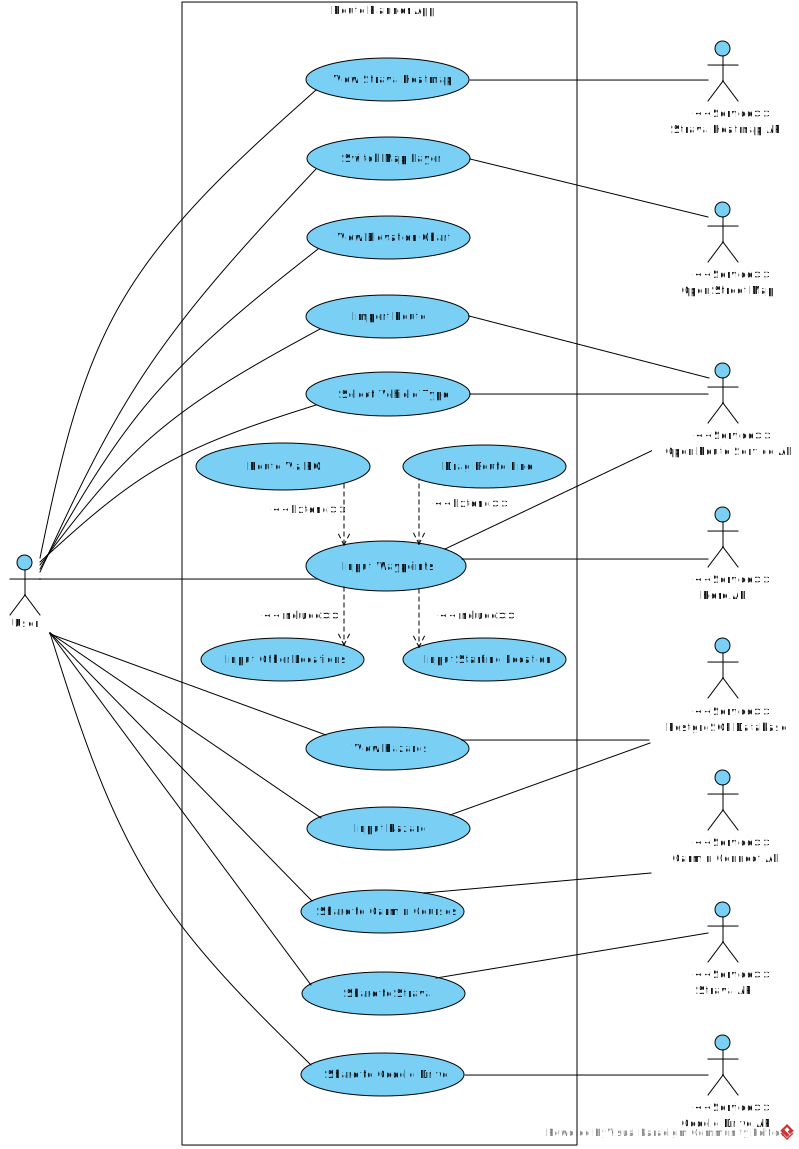
\includegraphics[width=400px]{figures/use-case.png}
  \caption{Use Case Diagram}
  \label{fig:usecase}
\end{figure}

\section{System Design}
\label{design:system}

\subsection{Architecture Design}
\label{system:architecture-design}

\subsection{Module Architecture}
\label{system:module-architecture}

\section{Critique of Designs}
\label{design:critique}
\chapter{Implementation}
\label{chap:implementation}

This section describes the artefact development process. Despite multiple stumbling blocks during development, these were overcome through problem-solving, thorough investigation and reading of software documentation.  

\section{Development Environment}
\label{implementation:de}

Visual Studio Code (VS Code) was chosen as the development environment for development (\cite{noauthor_visual_nodate}). VS Code was chosen due to its flexibility in working with multiple programming languages through the use of extensions. The React.js Framework, JavaScript and Go Language extensions were installed to ensure seamless development of the backend and frontend of the artefact. The ESLint extension was also used using Go and JavaScript configurations to ensure the consistency and readability of the codebase.

\section{Iteration 1 - Basic UI and Core Routing}
\label{implementation:iteration1}
The initial stages of development began using a first draft of elicited requirements \see{appendix:initial-user-requirements} where later in the project, a new set of user requirements was formed based on primary research. This method proved effective in not delaying initial development, where the core requirements were unlikely to change greatly. Furthermore, Iteration 1 consisted of implementing the building blocks of the artefact, including setting up a React.js App, Gin Webserver, PostgreSQL database and the core routing functionalities.

\subsection{Leaflet - Open Street Map (OSM)}
\label{iteration1:leaflet-osm}
The Map component was the first to be developed because the rest of the artefact would be dependent on its mapping functionality. The component contained a div element containing the MapContainer component imported from React Leaflet (\cite{noauthor_react_nodate}). The component includes a tile layer to make API requests to Open Street Map (\cite{noauthor_openstreetmap_nodate}) to get the tile images for the map, and then display these tiles to form the full-screen map element. Temporary variables were set up to store the latitude and longitude values representing the start and end of a route, then drawn on the map using a polyline and marker points \see{fig:basic-map-with-route}. 

\begin{figure}[!ht]
    \centering
    \includegraphics[width=425px]{figures/Progress Images/Iteration-1/SR25/Basic Route.png}
    \caption{Basic Map with Route}
    \label{fig:basic-map-with-route}
\end{figure}

\subsection{Basic Route Planning}
\label{iteration1:basic-routing}
After conducting research, the most effective way to implement route planning with Leaflet was to use Leaflet Routing Machine (\cite{noauthor_leaflet_nodate-1}). This library enabled a RoutingMachine component to be natively added on top of the React Leaflet map component, whilst providing a basic, customisable route planning UI \see{fig:routing-ui}. The routing API in use at the beginning was Open Source Routing Machine (OSRM) (\cite{noauthor_project_nodate}) which appeared to meet all requirements of a routing algorithm until round trip routing was required \see{iteration3:round-trip}. This new routing functionality enabled the user to select a start, destination and any intermediate locations, a route would then be planned. At this stage, the route could be altered through the use of waypoints, but the artefact did not provide any further custom routing features to the user.
\begin{figure}[!ht]
    \centering
    \includegraphics[width=425px]{figures/Progress Images/Iteration-1/SR1/Basic Destination Overlay Set up.png}
    \caption{Routing UI}
    \label{fig:routing-ui}
  \end{figure}

\subsection{Elevation Chart}
\label{iteration1:elevation-chart}
To create an elevation chart, the component was declared, with the plan to use Chart.js (\cite{noauthor_chartjs_nodate}) to draw the plot on a canvas element. A div was created to hold the chart component, where the elevation data was gathered from a state variable called 'coordinates' which contained the route latitude, longitude points and the altitude/elevations for each point \see{fig:waypoint-arr}. The distance along the route for each elevation point is calculated by dividing the total route distance (taken from a state variable called 'summary') by the length of the 'coordinates' array. To ensure continuity between the map and the elevation plot, a simple feature was added to allow the user to hover over the elevation plot, with the matching point along the route being highlighted. This required the hover point on the chart's canvas element to be found, matching the hover value to the latitude and longitude with the respective point and drawing a circle element on the Leaflet map \see{fig:elevation-hover}.

\begin{figure}[!ht]
    \centering
    \includegraphics[width=200px]{figures/Progress Images/Iteration-1/SR1/waypoint-arr.png}
    \caption{Route Waypoint/Elevation Array}
    \label{fig:waypoint-arr}
  \end{figure}

\begin{figure}[!ht]
    \centering
    \includegraphics[width=425px]{figures/Progress Images/Iteration-1/SR28/elevation-hover.png}
    \caption{Elevation Plot Hover Functionality}
    \label{fig:elevation-hover}
\end{figure}

\subsection{Weather Information Panel}
\label{iteration1:weather-panel}
A generic weather panel was created within iteration 1, displaying weather information for the current day at the user's current location. The weather panel used the browser's geolocation API called within a React useEffect to get the user's general location, asking for permission via a pop-up window, then storing the geolocation in a state variable. The approximate coordinates returned from the API were then passed to Open Weather Map to gather all weather data for the current day. The Meteocons icons (\cite{noauthor_weather_nodate}) were used to display images demonstrating the current weather conditions \see{fig:basic-weather-panel}. The visibility of the weather panel was determined by a State variable, if the variable was true, the height and width of the panel expand, and when false, reduce to the button size.

\begin{figure}[!ht]
    \centering
    \includegraphics[width=300px]{figures/Progress Images/Iteration-1/SR19&SR28 Combined/SR19&SR28 Merged.png}
    \caption{Weather Panel}
    \label{fig:basic-weather-panel}
\end{figure}

\subsection{Main Challenges}
\label{iteration1:main-challenges}
The main challenge of Iteration 1 (i1), was primarily integrating multiple services to communicate seamlessly through the React.js frontend. Syncing hovering over the elevation plot, with a matching point along the route polyline, proved difficult. Despite the calculations being simple to determine at what latitude and longitude to draw the circle marker on the map when hovering on the plot, getting the map instance reference was more difficult than expected. Initially, the reference would return undefined, therefore no marker was drawn on the map, however after implementing a useState and declaring a local copy of the map instance, the hover functionality worked seamlessly.

Furthermore, the only other challenge faced was retrieving the user's geolocation from the browser. A useEffect was required to access the geolocation API, however, the useState was at first missed to store the geolocation value once the API had returned the data. Once the state variable was added, however, the weather panel would re-render once the data was retrieved.

\section{Iteration 2 - Route Sharing, Hazard Index and POI Integration}
\label{implementation:iteration2}

Unlike i1, Iteration 2 (i2) development was conducted after the primary research and requirements review had been completed. The remaining updated requirements were prioritised and distributed between i2 and Iteration 3 (i3) \see{implementation:iteration3}. I2 builds on i1, enhancing existing functionality and introducing new features throughout the iteration. 

\subsection{Sharing Route Functionality}
\label{iteration2:sharing-route}

Route sharing was implemented with i2, when routes were found using Open Route Service, GPX (\cite{noauthor_gpx_nodate}) and GeoJSON (\cite{noauthor_geojson_nodate}) strings were generated. These files were then used to create a share to email feature using the Twilio SENDGRID API (\cite{noauthor_email_nodate}). Initially, it was planned to send emails direct to the SENDGRID directly from the client, to mitigate the middle-man required to send the request, however it was found that SENDGRID would only accept incoming requests from the server. Therefore, an API endpoint was created with Gin to handle the POST request from the frontend. 

Each email would contain a simple amount of predefined text with the included GPX and/or GeoJSON files selected for export. A modal was created to display the email form, where the user could input the recipient's email address, route name and choose what type of file to share \see{fig:basic-weather-panel}.

Initially, it was planned to use the Strava API to upload GPX files directly to the user's Strava Routes account, however, it was found that the Strava API had no such endpoint to integrate with routes. It was decided to still implement Strava integration, but with activities, enabling route export as an activity for users without dedicated fitness devices. 

A modal was created \see{fig:strava-modal} and a POST request endpoint set up to handle the request to the Strava API. The user would be required to log in to their Strava account, to enable the artefact access to upload activities. Once logged in, the user could select the route to upload, then the artefact would send the GPX file to the Strava API, where it would be converted to an activity and stored in the user's account \see{fig:strava-example}.

\begin{figure}[!ht]
  \centering
  \includegraphics[width=425px]{figures/Progress Images/Iteration-2/SR17/SR17png.png}
  \caption{Share to Email Modal}
  \label{fig:share-email-modal}
\end{figure}

\begin{figure}[!ht]
  \centering
  \includegraphics[width=425px]{figures/Progress Images/Iteration-2/SR18/SR18 Upload Example 1.png}
  \caption{Strava Activity}
  \label{fig:strava-example}
\end{figure}

\begin{figure}[!ht]
  \centering
  \includegraphics[width=425px]{figures/Progress Images/Iteration-2/SR18/SR18 Strava Modal.png}
  \caption{Share to Strava Modal}
  \label{fig:strava-modal}
\end{figure}


\subsection{Hazard Index Database Creation and Integration}
\label{iteration2:hazard-index}

Creation and integration of the hazard index database was the largest task of i2. The database was created using PostgreSQL using PostGIS. The database was split into eight tables representing a hazard, related details and its geospatial data \see{system:database-design}. Hazard types were chosen based on the most relevant hazards defined on the Open Street Map wiki (\cite{noauthor_keyhazard_nodate}) with the addition of a 'Cycling Infrastructure' hazard. The 'Cycling Infrastructure' hazard type was added to allow users to report and view bad cycling infrastructure in their area, with the intention of routing algorithms avoiding these areas in the future.

To integrate the database into the artefact, API endpoints were created to handle GET and POST requests to the database. The database was connected to the Go backend using the 'github.com/lib/pq' package (\cite{noauthor_pq_nodate}), with Gin handling the routing of requests to the database. Using the fetch API, the frontend could make API calls, to add and retrieve hazards from the database, supplying coordinates for the hazard location/area and the hazard type \see{fig:hazard-creation}.

To enable users to contribute to the hazard index database, a UI was created using the Leaflet Draw API (\cite{noauthor_leaflet_nodate-2}). The API allowed a few controls to be added to the map, including buttons to draw markers and polygons onto the map. These buttons were used to create a hazard, where I implemented an event handler to catch the polygon/marker drawn once completed. This event handler would then proceed to make open the hazard creation modal, with the coordinates of the drawn polygon/marker passed to the modal via props. The user could then add the extra information required for the hazard and submit the hazard to the database.

Furthermore, to display the hazard data on the map, a new layer must be created. The layer was added to the map using the React Leaflet library, where the hazards were retrieved from the database and drawn on the map. These hazards were shown as both markers and polygons to represent a point or area hazard \see{fig:hazard-layer}. The API endpoint was set up to allow the user to retrieve all hazards within a five mile radius of a point, to enable the user to see hazards in their area, as the map was panned, the hazard layer would update \see{fig:hazard-API}.

\begin{figure}[!ht]
  \centering
  \includegraphics[width=425px]{figures/Progress Images/Iteration-2/SR32-37/sr32-add-hazard-point.png}
  \caption{Hazard Creation Modal}
  \label{fig:hazard-creation}
\end{figure}

\begin{figure}[!ht]
  \centering
  \includegraphics[width=300px]{figures/Progress Images/Iteration-2/SR32-37/sr32-hazard-popup.png}
  \caption{Hazard Map Layer}
  \label{fig:hazard-layer}
\end{figure}

\begin{figure}[!ht]
  \centering
  \includegraphics[width=425px]{figures/Progress Images/Iteration-2/SR32-37/SR32 - Basic API further developed.png}
  \caption{Hazard API Query}
  \label{fig:hazard-API}
\end{figure}

\subsection{Key Point-of-Interest (POI) Integration}
\label{iteration2:poi-integration}

The POI integration was the final feature of i2, where the user could view points of interest in their area. The POI data was retrieved from the Foursquare Places API (\cite{noauthor_places_nodate}). Two separate map layers were created similar to the hazard layer \see{iteration2:hazard-index}, one to display accommodation POI and another to display the attractions/leisure POI \see{fig:poi-layers}. The layer also allowed the user to click on each POI marker to view more information about the location, such as the name and address.

After the core POI layers were developed, two buttons were then added to each POI popup window. These were to allow a user to either route to or via the POI. If the user chose to route to, the last route waypoint would be updated to the POI's latitude and longitude. Whereas to route via, the route waypoints would initially be taken to find which route waypoint was closest to the POI, it would then be inserted into waypoints before the closest waypoint. The route would then be recalculated to include the POI as a waypoint \see{fig:poi-route}.

\begin{figure}[!ht]
  \centering
  \includegraphics[width=425px]{figures/Progress Images/Iteration-2/SR40-45/SR40 - Attractions and Accommodation KeyPOI.png}
  \caption{Attractions and Accommodation Layers}
  \label{fig:poi-layers}
\end{figure}

\begin{figure}[!ht]
  \centering
  \includegraphics[width=425px]{figures/Progress Images/Iteration-2/SR40-45/SR45 - Route ToVia POI.png}
  \caption{Route To/Via POI}
  \label{fig:poi-route}
\end{figure}

\subsection{Main Challenges}
\label{iteration2:main-challenges}

The main challenges for i2 resided in setting up the SQL queries to handle the hazard data requests as well as oauth authentication with the Strava API.

The INSERT hazard query was the most complex. The PLpgSQL language was used to create a function to handle  this logic as loops were required when inserting multiple PostGIS Point data types (coordinates) for each hazard. A loop was also required to insert the properties for each hazard, where each hazard could have one or more. The function was then called from the API endpoint, passing the json string input directly into the PLpgSQL function as type JSONB.

The Strava API was also challenging as it was required to implement oAuth 2.0 manually to authorise the application to upload activities to the user's account. The Strava API documentation was relatively clear on how to implement this process, however, having not manually implemented oAuth before, without using libraries such as Auth0, it was a steep learning curve. This experience proved great later on however when implementing oAuth 1.0 for use with the Garmin Connect API \see{iteration3:garmin-integration}.


\clearpage
\section{Iteration 3 - Round Trip, Route Import and Garmin Integration}
\label{implementation:iteration3}

Finally, i3 included the remainder of the critical and desired requirements. These included round trip routing, route import, Garmin Connect integration and social media sharing. There were only a few requirements which were not implemented due to time constraints, these were lowest priority requirements and were not critical to the artefact's functionality.

\subsection{Round Trip Routing}
\label{iteration3:round-trip}

The OpenRouteService (ORS) API was implemented shortly after it was found that OSRM didn't support round-trip routing, only A to B routing \see{iteration1:basic-routing}. The new API was implemented towards the end of i1 ahead of knowing the requirements for i3. 

To implement round-trip, the library used for using ORS with Leaflet Routing Machine (\cite{noauthor_gegewebleaflet-routing-machine-openroute_2020}) was customised to fit the artefacts needs. A fork was created 'jaketbailey/leaflet-routing-machine-openroute' to allow the round trip feature to be used with the library. This fork allowed for only one waypoint to act as an input to trigger the API call for round trip routing. The API call would then return a route in the same format as an A to B route, with the start and end being the same point. The route was then drawn on the map and the elevation chart updated to reflect the new route \see{fig:round-trip}.

Once the updates were made to the forked library, the other functionalities of the artefact all worked seamlessly in both the standard A to B and the round trip mode. The only minor change required was to track the mode which the user last left the artefact in LocalStorage. This then ensured that when the user returned and chose to load their previous route, the artefact would know which mode to load the route and UI in.

\begin{figure}[!ht]
  \centering
  \includegraphics[width=425px]{figures/Progress Images/Iteration-3/SR11/SR11- Round Trip functionality working.png}
  \caption{Round Trip Route}
  \label{fig:round-trip}
\end{figure}

\subsection{Route Import}
\label{iteration3:route-import}

Importing routes was a vital feature as it would enable route sharing across many applications supporting the same standards. The GPX and GeoJSON file formats were chosen to be supported as they are the most common file formats used for route sharing and were already used for exporting routes from the artefact. Adding such a minor feature would enable the artefact to manually import routes from other applications, such as Strava, Komoot and RideWithGPS.



\subsection{Garmin Connect Integration}
\label{iteration3:garmin-integration}

\subsection{Social Media Sharing}
\label{iteration3:social-sharing}

\subsection{Main Challenges}
\label{iteration3:main-challenges}

\chapter{Testing}
\label{chap:testing}

This chapter outlines the process of testing with React.js and Go. The chapter will also cover the use of Postman for API testing and Chrome Developer Tools for debugging and testing in the browser.

\section{Unit Testing}
\label{testing:unit}

For unit testing, two frameworks were used. For the Go/Gin backend, the built-in Go test framework was used. For the React.js front, the Jest testing framework was used. The respective plugins were installed in VS Code to allow for easy running and visualisation of the tests \see{fig:unit-tests}.

Multiple tests were written to test the API GET endpoints. The tests were run via the aforementioned VS Code plugin or the terminal using the command `\texttt{go test}'. Using mock data inputs, the tests were written to ensure that the correct JSON object was returned in the correct format to be exploited by the front end.

Testing React.js components was a more complex process than writing tests for vanilla JavaScript. As the tests were required to be on a component-level basis, snapshot testing was used to ensure that the components were rendered correctly. To create a snapshot test, all data required by the component was mocked, including required functions. These functions were mocked using `\texttt{jest.fn}', `\texttt{jest.spyOn}' and `\texttt{mockImplementation}'. MockImplementation was used to mock the ChartJs Chart function, to ensure that the ElevationChart snapshot test was consistent with the actual component. To run the tests, either the command `\texttt{npm test}' or the VS Code plugin was used to run the tests.

\begin{figure}[!ht]
    \centering
    \includegraphics[width=150px]{figures/unit-tests.png}
    \caption{Unit Tests}
    \label{fig:unit-tests}
  \end{figure}

Manual unit tests were also conducted on the front end to ensure that the components behaved as expected. This was done by running the application and manually testing the components to ensure that they rendered correctly and that the data was displayed as expected \see{tab:unit-test-results}.

\begin{table}
\caption{Manual Unit Test Results}
\label{tab:unit-test-results}
\renewcommand{\arraystretch}{1.5} % Adjust the factor to suit your needs
\begin{tabular}{ p{1.85cm} p{10cm}  p{1.85cm} }
\hline
Test Case & Description & Pass?\\
\hline
 & \multicolumn{2}{p{11.85cm}}{\textbf{ElevationChart Component}}\\
01 & The component was tested to ensure that it renders correctly on load. & Y\\
02 & The component was tested to ensure that it renders correctly when changing the route. & Y\\
03 & The component was tested to ensure that it renders correctly when zooming into the chart. & Y\\
04 & The component was tested to ensure that it renders correctly when clicking reset zoom. & Y\\
\hline
 & \multicolumn{2}{p{11.85cm}}{\textbf{RoutingMachine Component}}\\
05 & The component was tested to ensure that it renders correctly on load. & Y\\
06 & The component was tested to ensure that it renders correctly when the waypoints are updated. & Y\\
07 & The component was tested to ensure that it renders correctly when the waypoints are dragged. & Y\\
08 & The component was tested to ensure that it renders correctly when the waypoints are removed. & Y\\
\hline
 & \multicolumn{2}{p{11.85cm}}{\textbf{WeatherPanel Component}}\\
09 & The component was tested to ensure that it renders correctly on load. & Y\\
10 & The component was tested to ensure that it renders correctly when the user shares their geolocation. & Y\\
\hline
 & \multicolumn{2}{p{11.85cm}}{\textbf{SharePanel Component}}\\
11 & The component was tested to ensure that it renders correctly on load. & Y\\
12 & The component was tested to ensure that it renders correctly when the share button is pressed. & Y\\
\hline
 & \multicolumn{2}{p{11.85cm}}{\textbf{RoutePreferencesPanel Component}}\\
13 & The component was tested to ensure that it renders correctly on load. & Y\\
14 & The component was tested to ensure that it renders correctly when the route preferences button is pressed. & Y\\
\end{tabular}
\end{table}

\section{Postman}
\label{testing:postman}

Postman was also used extensively through development to test the API. It was used to test the GET and POST endpoints to ensure that the correct data was being returned and that the correct data was being sent to the backend. In addition to testing the Go backend, Postman was also used to build and test API requests for Strava, Garmin Connect, Open Weather Map, Foursquare and the Here API. This was done to ensure that the API requests were being built correctly before being implemented into the artefact.

\section{Chrome Developer Tools}
\label{testing:chrome-dev}

The Chrome Developer Tools were also used to test the front end during development. The debugger was used to ensure that the JavaScript was running correctly and that the data was being passed correctly between the front and back end. Logs and breakpoints were also used to track the flow of data through the front end, ensuring that the state was being updated correctly and that the correct data was being passed to the components.
\chapter{Evaluation}
\label{chap:evaluation}

\section{Evaluation Methods and Techniques}
\label{evaluation:methods-and-technicques}

\section{Evaluation Process}
\label{evaluation:process}

\section{Evaluating Requirements}
\label{evaluation:requirements}

\section{Limitations}
\label{evaluation:limitations}

\section{Future Work}
\label{evaluation:future}
\chapter{Reflection and Conclusion}
\label{chap:reflection-and-conclusion}

\label{reflection-and-conclusion:what-went-well}
\section{What Went Well}

\label{reflection-and-conclusion:what-didnt-go-well}
\section{What Didn't Go Well}

\label{reflection-and-conclusion:outcomes/objectives-met}
\section{Were Outcomes and Objectives Met}

\label{reflection-and-conclusion:final-conclusion}
\section{Final Conclusion}



%%%%%%%%%%%%%% REFERENCES SECTION
\newpage
\phantomsection
\addcontentsline{toc}{chapter}{References}
% In order to try and get a consistent format I copy and paste the INSPIRE bibtex code into my bibtex file.
\printbibliography

%%%%%%%%%%%% Include your appendices here

\appendix
\chapter{Appendix}
\begin{figure}[!h]
    \centering
    \includegraphics[width=1\linewidth]{figures/plotarouteui.png}
    \caption{Plotaroute.com UI}
    \label{fig:plotarouteui}
\end{figure}

\begin{figure}[!h]
    \centering
    \includegraphics[width=1\linewidth]{figures/komootui.png}
    \caption{Komoot UI}
    \label{fig:komootui}
\end{figure}

\begin{figure}[!h]
    \centering
    \includegraphics[width=1\linewidth]{figures/gmapsui.png}
    \caption{Google Maps UI}
    \label{fig:gmapsui}
\end{figure}



\end{document}
